\documentclass{article}
\usepackage[margin=1in]{geometry}
\usepackage{amsmath, amssymb, amsthm}
\usepackage{enumitem}


% Cases Environment
\newlist{Cases}{enumerate}{3}
\setlist[Cases]{leftmargin = .20in, label = {Case \arabic*.}, topsep = 5pt, itemindent = 13mm}

\usepackage{bm}
\usepackage{booktabs}
\usepackage[table, dvipsnames]{xcolor}
\usepackage{colortbl}


\newcolumntype{a}{>{\columncolor{white}}c}
\newcolumntype{e}{>{\columncolor{gray!20}}c}
\newcolumntype{d}{>{\columncolor{gray!40}}c}

% colored links
\usepackage{hyperref}
\hypersetup{
    colorlinks=true,
    linkcolor=blue,
    filecolor=magenta,      
    urlcolor=magenta,
    }

\newtheorem{claim}{Claim}

%Creating algorithms
\usepackage{algorithm}
\usepackage[noend]{algpseudocode}


%Images
\usepackage{graphicx}
    \usepackage{subcaption}
    \usepackage{float}
    % \usepackage[labelsep=period]{caption}


% Inputting Python code
% \usepackage[dvipsnames]{xcolor}
\definecolor{textblue}{rgb}{.2,.2,.7}
\definecolor{textred}{rgb}{0.54,0,0}
\definecolor{textgreen}{rgb}{0,0.43,0}
\usepackage{upquote}
\usepackage{listings}
\lstset{
    language=Python, 
    tabsize=4,
    basicstyle={\ttfamily},
    keywordstyle=\color{textblue},
    commentstyle=\color{textgreen},
    stringstyle=\color{textred},
    frame=none,
    columns=fullflexible,
    keepspaces=true,
    showstringspaces=false,
    xleftmargin=-15mm, % manual adjustment, figure out permanent solution
}

%Drawing Graphs
\usepackage{tikz}
    \usetikzlibrary{arrows}
    \usetikzlibrary{patterns}
    \usetikzlibrary{intersections}
\usepackage{pgfplots} \pgfplotsset{compat=newest} 
    \usepgfplotslibrary{fillbetween}

% Tcolorbox
\usepackage{tcolorbox}
\tcbuselibrary{skins,hooks}
\usetikzlibrary{shadows}

%Creating Figures
\usepackage{tikz}
\usetikzlibrary{calc, math, matrix, graphs, positioning}
\usetikzlibrary{fit}
\usetikzlibrary{backgrounds}
\usetikzlibrary{hobby}

% the settings of tikz is used for the optimization of the graphs  
\usetikzlibrary{shapes, arrows, arrows.meta} % these are the parameters passed to the library to create the node graphs  
\tikzset{  
    auto,node distance =1.1 cm and 1.1 cm,% node distance is the distance between one node to other, where 1.5cm is the length of the edge between the nodes  
} 

%Formatting and Spacing
\setitemize[1]{noitemsep, parsep = 5pt, topsep = 5pt}
\setenumerate[1]{label = (\alph*), parsep = 1pt, topsep = 5pt}
\setlength\parindent{0pt}
\linespread{1.1}

% title
\title{\vspace{-1cm}CS 2051: Honors Discrete Mathematics \\Spring 2023 \texttt{generate\_cfg\_tricky} Solution}
\author{Sarthak Mohanty}
\date{}


\begin{document}

\maketitle

In this document, we cover the solution to the \lstinline{generate_cfg_tricky} function. Recall that our goal in this function was to generate a context-free grammar (CFG) for the language $$L = \{1^{i}0^{j} : 2i \ne 3j + 1\}.$$ (Unless otherwise indicated, $i, j \in \mathbb{N}$ should always be assumed.)

\vspace{2mm}Let's kick off our analysis by exploring the language from a geometric perspective. First, map each string of the form $1^{i}0^{j}$ to points in a discrete 2D space, where the $x$-axis represents the number of 1's ($i$) and the $y$-axis represents the number of 0's ($j$). Next, consider the \textit{complement} of language $L$: $$\bar{L} = \{1^{i}0^{j} : 2i = 3j + 1\}.$$ If we view these two languages through the lens of a \textbf{linear classification} problem, the linear condition for $\bar{L}$ (i.e., $2i = 3j + 1$) can be seen as a decision boundary that separates points in the 2D space. With this in mind, the language $L$ can be seen as the set of regions that result from this decision boundary, as depicted in Figure (\ref{fig:cfg}).

\vspace{2mm}
This new interpretation also gives us a strategy for generating $L$: construct a CFG for each of the two halfspaces, then combine them to create a CFG deciding their union. Before we start this process, though, we'll make a quick detour to create a CFG for $\bar{L}$, as the techniques used to do so are similar to those in the primary construction.

\begin{figure}[htbp]
    \centering
    \captionsetup{width=.8\linewidth}
    \begin{subfigure}{0.45\textwidth}
        \centering
        \captionsetup{width=.8\linewidth}
        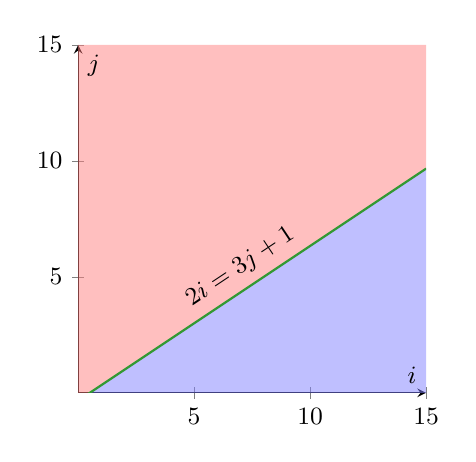
\begin{tikzpicture}[font=\small]
        \begin{axis}[
            width=6cm, height=6cm,
            axis lines = center,
            xlabel=$i$,
            ylabel=$j$,
            xmin = 0, xmax = 15,
            ymin = 0, ymax = 15,
        ]
        % Red region
        \fill[red!50, fill opacity=0.5] (axis cs:0,0) -- (axis cs:0,15) -- (axis cs:15,15) --(axis cs:15,29/3) --(axis cs:1/2,0) -- cycle;
        
        % Blue region
        \fill[blue!50, fill opacity=0.5] (axis cs:1/2,0) -- (axis cs:15,0) -- (axis cs:15,29/3) -- cycle;

        \addplot [smooth, name path=a, Green!80, thick, domain = 0:15] (x, x*2/3-1/3) node [sloped, midway, above, black] {$2i = 3j + 1$};
        \end{axis}
        \end{tikzpicture}
        \caption{Decision boundary applied to the Cartesian plane.}
    \end{subfigure}
    \begin{subfigure}{0.45\textwidth}
        \centering
        \captionsetup{width=.8\linewidth}
        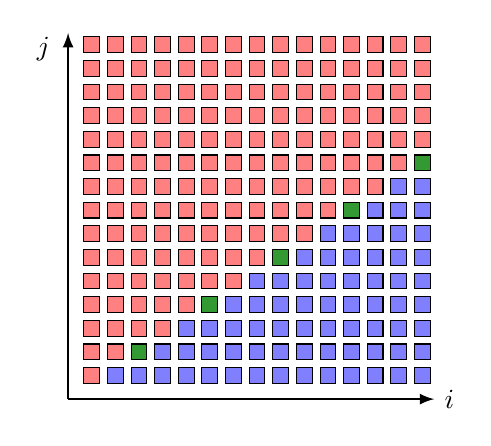
\begin{tikzpicture}[scale=0.3]
            \foreach \i in {0,...,14} {
                \foreach \j in {0,...,14} {
                    \pgfmathparse{abs(2*\i - 3*\j - 1) < 0.1 ? 1 : (2*\i > 3*\j + 1 ? 2 : 0)}
                    \ifnum\pgfmathresult=1
                        \edef\nodecolor{Green!80}
                    \else
                        \ifnum\pgfmathresult=2
                            \edef\nodecolor{blue!50}
                        \else
                            \edef\nodecolor{red!50}
                        \fi
                    \fi
                    \node[rectangle, draw, fill=\nodecolor, minimum width=0.2cm, minimum height=0.2cm, inner sep=0pt] at (\i+0.5, \j+0.5) {};
                }
            }
            % Draw axes (bottom left)
            \draw[-latex, thick] (-0.5, -0.5) -- (15, -0.5) node[anchor=west] {$i$};
            \draw[-latex, thick] (-0.5, -0.5) -- (-0.5, 15) node[anchor=east,yshift=-2mm,xshift=-1mm] {$j$};
            % \node at (15, -0.5) [anchor=west] {\phantom{$i$}};
            % \node at (-0.5, 15) [anchor=south] {\phantom{$j$}};
            
        \end{tikzpicture}
        \caption{Decision boundary applied to a 2D grid representing the strings in the language.}
        \label{fig:grid_cfg}
    \end{subfigure}
    \caption{Geometric visualization of languages $L$ and $\bar{L}$: the decision boundary $2i = 3j + 1$ divides the plane into two distinct halfspaces.}
    \label{fig:cfg}
\end{figure}



\section*{Warm-up: CFG for $\bm{\bar{L}} = \bm{\{1^{i}0^{j} : 2i = 3j + 1\}}$}
    First, let's look at the values for $i, j$ that satisfy our conditions. From Figure (\ref{fig:grid_cfg}), we can amass the following table of values:
    $$\begin{array}{c|ccccc}
        \toprule
        i & 2 & 5 & 8 & 11 & 14 \\
        \midrule
        j & 1 & 3 & 5 & 7 & 9 \\
        \bottomrule
    \end{array}$$
    A pattern begins to emerge: three right, two up, three right, two up \dots. Already we can guess that any satisfactory string $1^{i}0^{j}$ must be of the form $1^{3k + 2}0^{2k + 1}$. We can prove it as well!

    \vspace{2mm}
    \textbf{Claim:} Let $k \in \mathbb{N}$. Then $$\left\{1^{i}0^{j} : 2i = 3j + 1\right\} = \left\{1^{3k + 2}0^{2k + 1}\right\}.$$
    \begin{proof}
        $(\subseteq)$ The condition $2i = 3j + 1$ tells us that $3j + 1$ is an even number, which in turn implies $j$ is odd. Thus by definition, $j = 2k + 1$ for some $k \in \mathbb{N}$. Plugging this back into the original condition, we obtain $$2i = 3(2k + 1) + 1 \implies i = 3k + 2.$$
        $(\supseteq)$ Suppose $i = 3k + 2$ and $j = 2k + 1$. Then $$2i = 2(3k + 2) = 6k + 4 = 3(2k + 1) + 1 = 3j + 1.$$
    \end{proof}
    Now generating a CFG for $\bar{L} = \left\{1^{3k + 2}0^{2k + 1}\right\}$ is easy:
    $$S \rightarrow 111S000 \mid 11S0.$$

\section*{Main Result: A CFG for $\bm{L = \{1^{i}0^{j} : 2i \ne 3j + 1\}}$}
    We generate a CFG for $L$ using the strategy mentioned in the beginning of the document. To be specific, we split up $L$ as $$L = \underbrace{\{1^{i}0^{j} : 2i > 3j + 1\}}_{L_{1}} \ \cup \ \underbrace{\{1^{i}0^{j} : 2i < 3j + 1\}}_{L_{2}}$$ and generate CFGs for $L_{1}$ and $L_{2}$.

\subsection*{Part 1: CFG for $\bm{L_{1} = \{1^{i}0^{j} : 2i > 3j + 1\}}$}
    Similar to the warm-up, we first convert our language into a more manageable form. Consider the set $$M_{1} = \{(i, j) \in L_{1} : \nexists (i', j) \in L_{1} \text{ such that } i' < i\}.$$ In simpler terms, $M_{1}$ consists of the "leftmost" (closest to the $j$-axis) cells in $L_{1}$. Writing these values down, we get the following table:
    $$\begin{array}{c | a  e  a  e  a  e  a  e  a  }
        \toprule
        i & 1 & 3 & 4 & 6 & 7 & 9 & 10 & 12 & 13 \\
        \midrule
        j & 0 & 1 & 2 & 3 & 4 & 5 & 6 & 7 & 8 \\
        \bottomrule
    \end{array}$$
    A new pattern begins to emerge (based on the parity of $j$): we see the same staircase pattern as in $\bar{L}$, except now it is repeated twice! In particular, we claim that any $(i, j) \in M_{1}$ is of the form $(3k + 1, 2k)$ or $(3k + 3, 2k + 1)$. In turn, this implies any $1^{i}0^{j} \in L_{1}$ is of the form $1^{3k + 1 + c}0^{2k}$ or $1^{3k + 3 + c}0^{2k + 1}$. An illustration of this is shown in Figure (\ref{fig:cfg_part1}). \footnote{At this point, if I were a student, I would go straight to constructing the appropriate CFG. Woefully, I am not a student anymore!}
    
    \vspace{2mm}
    \textbf{Claim. } Let $k, c \in \mathbb{N}$. Then $$\left\{1^{i}0^{j} : 2i < 3j + 1\right\} = \left\{1^{3k + 1 + c}0^{2k}\right\} \cup \left\{1^{3k + 3 + c}0^{2k + 1}\right\}.$$
    \begin{proof}
        $(\subseteq)$ Suppose we have a string that satisfies the inequality $2i > 3j + 1$. Rewriting in terms of $i$, we have $i > \frac{3}{2}j + \frac{1}{2}$. We now have two cases based on the parity of $j$.
        
        \begin{Cases}
            \item Suppose $j$ is even. Then by definition, $j = 2k$ for some $k \in \mathbb{Z}$. Plugging this into the condition, we have $i > 3k + \frac{1}{2}$. Since $i$ must be an integer, the smallest value for $i$ that satisfies this inequality is $i = 3k + 1$. Then we have $i = 3k + 1 + c$, for some natural number $c$. In this case, the string is of the form $1^{3k + 1 + c}0^{2k}$.
            \item Suppose $j$ is odd. Then it can be written as $j = 2k + 1$, so we can express the inequality as $i > 3k + \frac{3}{2}$. The smallest value for $i$ satisfying this inequality is $i = 3k + 2$. Therefore, any $i$ can be expressed in the form $i = 3k + 2 + c$, for some $c \in \mathbb{N}$. In this case, the string is of the form $1^{3k + 3 + c}0^{2k + 1}$.
        \end{Cases}
        $(\supseteq)$ If $i = 3k + 1 + c$ and $j = 2k$, then $$2i = 2(3k + 1 + c) = 6k + 2 + 2c > 6k + 1 = 3(2k) + 1 = 3j + 1.$$ On the other hand, if $i = 3k + 3 + c$ and $j = 2k + 1$, then $$2i = 2(3k + 3 + c) = 6k + 6 + 2c > 6k + 4 = 3(2k + 1) + 1 = 3j + 1.$$
    \end{proof}
    We can now directly convert this alternate formulation of $L_{1}$ into a context-free grammar: 
    \begin{align*}
        S &\rightarrow S_{1} \mid S_{2} \\
        S_{1} &\rightarrow 111S_{1}00 \mid 1S_{1} \mid 1 \\
        S_{2} &\rightarrow 111S_{2}00 \mid 1S_{2} \mid 1110
    \end{align*}
    \begin{figure}[htbp]
        \centering
        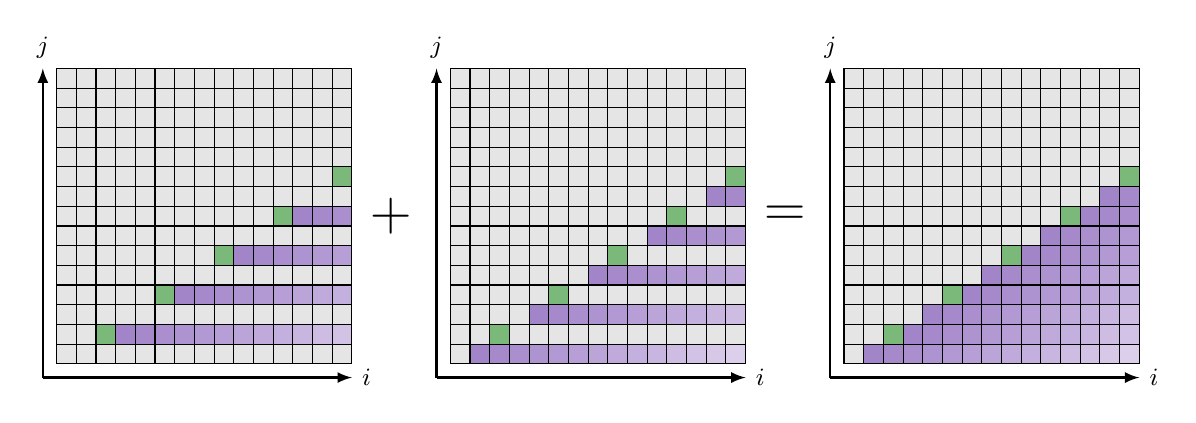
\begin{tikzpicture}[scale=0.25, font=\small]
            \begin{scope}[local bounding box=fig1]
                \foreach \i in {0,...,14} {
                    \foreach \j in {0,...,14} {
                        \pgfmathparse{abs(2*\i - 3*\j - 1) < 0.1 ? 1 : (2*\i > 3*\j + 1 ? 2 : 0)}
                        \ifnum\pgfmathresult=1
                            \edef\nodecolor{ForestGreen!60}
                        \else
                            \edef\nodecolor{gray!20}
                        \fi
                        \node[rectangle, draw, fill=\nodecolor, minimum width=0.25cm, minimum height=0.25cm, inner sep=0pt] at (\i+0.5, \j+0.5) {};
                    }
                }
                \foreach \k in {0,...,3} {
                    \pgfmathtruncatemacro{\maxone}{14-(3*\k+3)}
                    \foreach \x in {0,...,\maxone} {
                        \pgfmathsetmacro{\colorIntensity}{50 * (1 - \x / 20)}
                        \node[rectangle, draw, fill=RoyalPurple!\colorIntensity, minimum width=0.25cm, minimum height=0.25cm, inner sep=0pt] at (3*\k+3+0.5+\x, 2*\k+1+0.5) {};
                    }
                }
                \draw[-latex, thick] (-0.7, -0.7) -- (15, -0.7) node[anchor=west] {$i$};
                \draw[-latex, thick] (-0.7, -0.7) -- (-0.7, 15) node[anchor=south] {$j$};
            \end{scope}
            
            \node[font=\huge] at (17, 7.5) {+};
            
            \begin{scope}[shift={(20,0)}, local bounding box=fig2]
                \foreach \i in {0,...,14} {
                    \foreach \j in {0,...,14} {
                        \pgfmathparse{abs(2*\i - 3*\j - 1) < 0.1 ? 1 : (2*\i > 3*\j + 1 ? 2 : 0)}
                        \ifnum\pgfmathresult=1
                            \edef\nodecolor{ForestGreen!60}
                        \else
                            \edef\nodecolor{gray!20}
                        \fi
                        \node[rectangle, draw, fill=\nodecolor, minimum width=0.25cm, minimum height=0.25cm, inner sep=0pt] at (\i+0.5, \j+0.5) {};
                    }
                }
                \foreach \k in {0,...,4} {
                    \pgfmathtruncatemacro{\maxtwo}{14-(3*\k+1)}
                    \foreach            \x in {0,...,\maxtwo} {
                        \pgfmathsetmacro{\colorIntensity}{50 * (1 - \x / 20)}
                        \node[rectangle, draw, fill=RoyalPurple!\colorIntensity, minimum width=0.25cm, minimum height=0.25cm, inner sep=0pt] at (3*\k+1+0.5+\x, 2*\k+0.5) {};
                    }
                }
                \draw[-latex, thick] (-0.7, -0.7) -- (15, -0.7) node[anchor=west] {$i$};
                \draw[-latex, thick] (-0.7, -0.7) -- (-0.7, 15) node[anchor=south] {$j$};
            \end{scope}
        
            \node[font=\huge] at (37, 7.5) {=};
        
            \begin{scope}[shift={(40,0)}, local bounding box=fig3]
                \foreach \i in {0,...,14} {
                        \foreach \j in {0,...,14} {
                            \pgfmathparse{abs(2*\i - 3*\j - 1) < 0.1 ? 1 : (2*\i > 3*\j + 1 ? 2 : 0)}
                            \ifnum\pgfmathresult=1
                                \edef\nodecolor{ForestGreen!60}
                            \else
                                \edef\nodecolor{gray!20}
                            \fi
                            \node[rectangle, draw, fill=\nodecolor, minimum width=0.25cm, minimum height=0.25cm, inner sep=0pt] at (\i+0.5, \j+0.5) {};
                        }
                    }
                \foreach \k in {0,...,3} {
                    \pgfmathtruncatemacro{\maxone}{14-(3*\k+3)}
                    \foreach \x in {0,...,\maxone} {
                        \pgfmathsetmacro{\colorIntensity}{50 * (1 - \x / 20)}
                        \node[rectangle, draw, fill=RoyalPurple!\colorIntensity, minimum width=0.25cm, minimum height=0.25cm, inner sep=0pt] at (3*\k+3+0.5+\x, 2*\k+1+0.5) {};
                    }
                }
                \foreach \k in {0,...,4} {
                    \pgfmathtruncatemacro{\maxtwo}{14-(3*\k+1)}
                    \foreach \x in {0,...,\maxtwo} {
                        \pgfmathsetmacro{\colorIntensity}{50 * (1 - \x / 20)}
                        \node[rectangle, draw, fill=RoyalPurple!\colorIntensity, minimum width=0.25cm, minimum height=0.25cm, inner sep=0pt] at (3*\k+1+0.5+\x, 2*\k+0.5) {};
                    }
                }
                \draw[-latex, thick] (-0.7, -0.7) -- (15, -0.7) node[anchor=west] {$i$};
                \draw[-latex, thick] (-0.7, -0.7) -- (-0.7, 15) node[anchor=south] {$j$};
            \end{scope}
        \end{tikzpicture}
        \caption{An alternative visualization of $L_{1}$}
        \label{fig:cfg_part1}
    \end{figure}

\subsection*{Part 2: CFG for $\bm{L_{2} = \{1^{i}0^{j} : 2i < 3j + 1\}}$}
    We employ a similar strategy as in Part 1: consider the set $M_{2}$ consisting of the ``bottom-most" elements in $L_{2}$. Formally, $$M_{2} = \{(i, j) \in L_{2} : \nexists (i, j') \in L_{2} \text{ such that } j' < j\}.$$ Again, we begin by writing values down:
    $$\begin{array}{c | a e d a e d a e d a e d a e d a e d}
        \toprule
        i & 0 & 1 & 2 & 3 & 4 & 5 & 6 & 7 & 8 \\
        \midrule
        j & 0 & 1 & 2 & 2 & 3 & 4 & 4 & 5 & 6 \\
        \bottomrule
    \end{array}$$
    Using the table, we guess that any string in $L_{2}$ must be of the form $1^{3k}0^{2k+c}$, $1^{3k+1}0^{2k+1+c}$, or $1^{3k+2}0^{2k+2+c}$ (Illustrated in Figure \ref{fig:cfg_part2}).

    \vspace{2mm}
    \textbf{Claim. } Let $k, c \in \mathbb{N}$. Then $$\{1^{i}0^{j} : 2i < 3j + 1\} = \left\{1^{3k}0^{2k+c}\right\} \cup \left\{1^{3k+1}0^{2k+1+c}\right\} \cup \left\{1^{3k+2}0^{2k+2+c}\right\}.$$

    \begin{proof}
        $(\subseteq)$ Suppose we have a string that satisfies the inequality $2i < 3j + 1$. Rewriting in terms of $j$ yields $j > \frac{2}{3}i - \frac{1}{3}$. We consider three cases, based on the value of $i \pmod{3}$:
        
        \begin{Cases}
            \item Suppose $i \pmod{3} = 0$. Then $i = 3k$ for some $k \in \mathbb{N}$. Plugging this into the condition above, we get $j > 2k - \frac{1}{3}$. The smallest integer value for $j$ satisfying this condition is $j = 2k$, so any satisfactory $j$ can be expressed in the form $j = 2k + c$, for some natural number $c$. 
            
            In this case, the string is of the form $1^{3k}0^{2k+c}$.
            \item Suppose $i \pmod{3} = 1$. Then $i = 3k + 1$ for some $k \in \mathbb{N}$. Plugging this into the condition above, we get $j > 2k + \frac{1}{3}$. The smallest integer value for $j$ satisfying this condition is $2k + 1$, any satisfactory $j$ is of the form $j = 2k + 1 + c$.
            
            In this case, the string is of the form $1^{3k + 1}0^{2k + 1 + c}$.
            \item Suppose $i \pmod{3} = 2$. Then $i = 3k + 2$ for some $k \in \mathbb{N}$. Plugging this into the condition above, we get $j > 2k + 1$. The smallest integer value for $j$ satisfying this condition is $2k + 2$, so any satisfactory $j$ is of the form $j = 2k + 2 + c$.
            
            In this case, the string is of the form $1^{3k + 2}0^{2k + 2 + c}$.
        \end{Cases}
        $(\supseteq)$ Left to the reader (similar to Part 1).
    \end{proof}
    Again, it is now easy to convert this language into a context-free grammar: 
    \begin{align*}
        S &\rightarrow S_{1} \mid S_{2} \mid S_{3} \\
        S_{1} &\rightarrow 111S_{1}00 \mid S_{1}0 \mid \epsilon \\
        S_{2} &\rightarrow 111S_{1}00 \mid S_{2}0 \mid 10 \\
        S_{3} &\rightarrow 111S_{2}00 \mid S_{3}0 \mid 1100
    \end{align*}
    
    \begin{figure}[htbp]
        \centering
        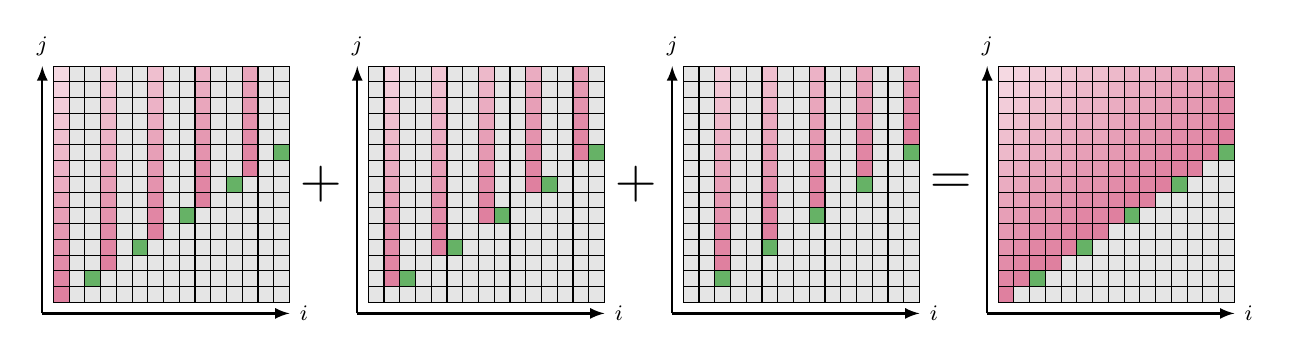
\begin{tikzpicture}[scale=0.2, font=\footnotesize]
            \begin{scope}[local bounding box=fig1]
                \foreach \i in {0,...,14} {
                    \foreach \j in {0,...,14} {
                        \pgfmathparse{abs(2*\i - 3*\j - 1) < 0.1 ? 1 : (2*\i > 3*\j + 1 ? 2 : 0)}
                        \ifnum\pgfmathresult=1
                            \edef\nodecolor{Green!60}
                        \else
                            \edef\nodecolor{gray!20}
                        \fi
                        \node[rectangle, draw, fill=\nodecolor, minimum width=0.2cm, minimum height=0.2cm, inner sep=0pt] at (\i+0.5, \j+0.5) {};
                    }
                }
                \foreach \k in {0,...,4} {
                    \pgfmathtruncatemacro{\maxone}{14-(2*\k)}
                    \foreach \y in {0,...,\maxone} {
                        \pgfmathsetmacro{\colorIntensity}{50 * (1 - \y / 20)}
                        \node[rectangle, draw, fill=purple!\colorIntensity, minimum width=0.2cm, minimum height=0.2cm, inner sep=0pt] at (3*\k+0.5, 2*\k+0.5+\y) {};
                    }
                }
                \draw[-latex, thick] (-0.7, -0.7) -- (15, -0.7) node[anchor=west] {$i$};
                \draw[-latex, thick] (-0.7, -0.7) -- (-0.7, 15) node[anchor=south] {$j$};
            \end{scope}
            
            \node[font=\huge] at (17, 7.5) {+};
            
            \begin{scope}[shift={(20,0)}, local bounding box=fig2]
                \foreach \i in {0,...,14} {
                    \foreach \j in {0,...,14} {
                        \pgfmathparse{abs(2*\i - 3*\j - 1) < 0.1 ? 1 : (2*\i > 3*\j + 1 ? 2 : 0)}
                        \ifnum\pgfmathresult=1
                            \edef\nodecolor{Green!60}
                            \else
                                \edef\nodecolor{gray!20}
                            \fi
                        \node[rectangle, draw, fill=\nodecolor, minimum width=0.2cm, minimum height=0.2cm, inner sep=0pt] at (\i+0.5, \j+0.5) {};
                    }
                }
                \foreach \k in {0,...,4} {
                    \pgfmathtruncatemacro{\maxtwo}{14-(2*\k+1)}
                    \foreach \y in {0,...,\maxtwo} {
                        \pgfmathsetmacro{\colorIntensity}{50 * (1 - \y / 20)}
                        \node[rectangle, draw, fill=purple!\colorIntensity, minimum width=0.2cm, minimum height=0.2cm, inner sep=0pt] at (3*\k+1+0.5, 2*\k+1+0.5+\y) {};
                    }
                }
                \draw[-latex, thick] (-0.7, -0.7) -- (15, -0.7) node[anchor=west] {$i$};
                \draw[-latex, thick] (-0.7, -0.7) -- (-0.7, 15) node[anchor=south] {$j$};
            \end{scope}
        
            \node[font=\huge] at (37, 7.5) {+};
        
            \begin{scope}[shift={(40,0)}, local bounding box=fig3]
                \foreach \i in {0,...,14} {
                        \foreach \j in {0,...,14} {
                            \pgfmathparse{abs(2*\i - 3*\j - 1) < 0.1 ? 1 : (2*\i > 3*\j + 1 ? 2 : 0)}
                            \ifnum\pgfmathresult=1
                                \edef\nodecolor{Green!60}
                            \else
                                \edef\nodecolor{gray!20}
                            \fi
                            \node[rectangle, draw, fill=\nodecolor, minimum width=0.2cm, minimum height=0.2cm, inner sep=0pt] at (\i+0.5, \j+0.5) {};
                        }
                    }
                \foreach \k in {0,...,4} {
                    \pgfmathtruncatemacro{\maxthree}{14-(2*\k+2)}
                    \foreach \y in {0,...,\maxthree} {
                        \pgfmathsetmacro{\colorIntensity}{50 * (1 - \y / 20)}
                        \node[rectangle, draw, fill=purple!\colorIntensity, minimum width=0.2cm, minimum height=0.2cm, inner sep=0pt] at (3*\k+2+0.5, 2*\k+2+0.5+\y) {};
                    }
                }
                \draw[-latex, thick] (-0.7, -0.7) -- (15, -0.7) node[anchor=west] {$i$};
                \draw[-latex, thick] (-0.7, -0.7) -- (-0.7, 15) node[anchor=south] {$j$};
                \end{scope}
        
            \node[font=\huge] at (57, 7.5) {=};
        
            \begin{scope}[shift={(60,0)}, local bounding box=fig4]
            \foreach \i in {0,...,14} {
                    \foreach \j in {0,...,14} {
                        \pgfmathparse{abs(2*\i - 3*\j - 1) < 0.1 ? 1 : (2*\i > 3*\j + 1 ? 2 : 0)}
                        \ifnum\pgfmathresult=1
                            \edef\nodecolor{Green!60}
                        \else
                            \edef\nodecolor{gray!20}
                        \fi
                        \node[rectangle, draw, fill=\nodecolor, minimum width=0.2cm, minimum height=0.2cm, inner sep=0pt] at (\i+0.5, \j+0.5) {};
                    }
                }
            \foreach \k in {0,...,4} {
    
                \pgfmathtruncatemacro{\maxone}{14-(2*\k)}
                \foreach \y in {0,...,\maxone} {
                    \pgfmathsetmacro{\colorIntensity}{50 * (1 - \y / 20)}
                    \node[rectangle, draw, fill=purple!\colorIntensity, minimum width=0.2cm, minimum height=0.2cm, inner sep=0pt] at (3*\k+0.5, 2*\k+0.5+\y) {};
                }
    
                \pgfmathtruncatemacro{\maxtwo}{14-(2*\k+1)}
                \foreach \y in {0,...,\maxtwo} {
                    \pgfmathsetmacro{\colorIntensity}{50 * (1 - \y / 20)}
                    \node[rectangle, draw, fill=purple!\colorIntensity, minimum width=0.2cm, minimum height=0.2cm, inner sep=0pt] at (3*\k+1+0.5, 2*\k+1+0.5+\y) {};
                }
                
                \pgfmathtruncatemacro{\maxthree}{14-(2*\k+2)}
                \foreach \y in {0,...,\maxthree} {
                    \pgfmathsetmacro{\colorIntensity}{50 * (1 - \y / 20)}
                    \node[rectangle, draw, fill=purple!\colorIntensity, minimum width=0.2cm, minimum height=0.2cm, inner sep=0pt] at (3*\k+2+0.5, 2*\k+2+0.5+\y) {};
                }
            }
            \draw[-latex, thick] (-0.7, -0.7) -- (15, -0.7) node[anchor=west] {$i$};
            \draw[-latex, thick] (-0.7, -0.7) -- (-0.7, 15) node[anchor=south] {$j$};
            \end{scope}
        \end{tikzpicture}
        \caption{An alternative visualization of $L_{2}$}
        \label{fig:cfg_part2}
    \end{figure}

\subsection*{Part 3: Putting it all Together}
    Now that we have generated CFGs for $L_{1}$ and $L_{2}$, we combine them together to create our CFG for $L$, as shown in Figure (\ref{fig:cfg_part3}). Our final CFG is
    \begin{align*}
        S &\rightarrow S_{1} \mid S_{2} \mid S_{3} \mid S_{4} \mid S_{5} \\
        S_{1} &\rightarrow 111S_{1}00 \mid 1S_{1} \mid 1 \\
        S_{2} &\rightarrow 111S_{2}00 \mid 1S_{2} \mid 1110 \\
        S_{3} &\rightarrow 111S_{3}00 \mid S_{3}0 \mid \epsilon \\
        S_{4} &\rightarrow 111S_{4}00 \mid S_{4}0 \mid 10 \\
        S_{5} &\rightarrow 111S_{5}00 \mid S_{5}0 \mid 1100
    \end{align*}
    There are ways to optimize this CFG so there are less variables, less rules, etc., but the main idea(s) should remain the same.

    \begin{figure}[htbp]
        \centering
        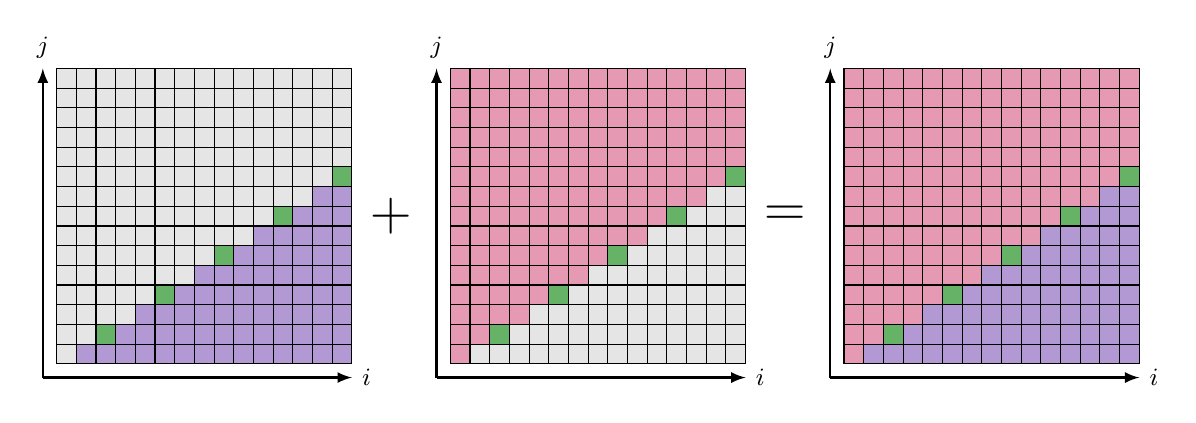
\begin{tikzpicture}[scale=0.25, font=\small]
            \begin{scope}[local bounding box=fig1]
                \foreach \i in {0,...,14} {
                        \foreach \j in {0,...,14} {
                            \pgfmathparse{abs(2*\i - 3*\j - 1) < 0.1 ? 1 : (2*\i > 3*\j + 1 ? 2 : 0)}
                            \ifnum\pgfmathresult=1
                                \edef\nodecolor{Green!60}
                            \else
                                \ifnum\pgfmathresult=2
                                    \edef\nodecolor{RoyalPurple!40}
                                \else
                                    \edef\nodecolor{gray!20}
                                \fi
                            \fi
                            \node[rectangle, draw, fill=\nodecolor, minimum width=0.25cm, minimum height=0.25cm, inner sep=0pt] at (\i+0.5, \j+0.5) {};
                        }
                    }
                \draw[-latex, thick] (-0.7, -0.7) -- (15, -0.7) node[anchor=west] {$i$};
                \draw[-latex, thick] (-0.7, -0.7) -- (-0.7, 15) node[anchor=south] {$j$};
                \end{scope}
            
            \node[font=\huge] at (17, 7.5) {+};
            
            \begin{scope}[shift={(20,0)}, local bounding box=fig2]
                \foreach \i in {0,...,14} {
                        \foreach \j in {0,...,14} {
                            \pgfmathparse{abs(2*\i - 3*\j - 1) < 0.1 ? 1 : (2*\i > 3*\j + 1 ? 2 : 0)}
                            \ifnum\pgfmathresult=1
                                \edef\nodecolor{Green!60}
                            \else
                                \ifnum\pgfmathresult=2
                                    \edef\nodecolor{gray!20}
                                \else
                                    \edef\nodecolor{purple!40}
                                \fi
                            \fi
                            \node[rectangle, draw, fill=\nodecolor, minimum width=0.25cm, minimum height=0.25cm, inner sep=0pt] at (\i+0.5, \j+0.5) {};
                        }
                    }
                \draw[-latex, thick] (-0.7, -0.7) -- (15, -0.7) node[anchor=west] {$i$};
                \draw[-latex, thick] (-0.7, -0.7) -- (-0.7, 15) node[anchor=south] {$j$};
            \end{scope}
        
            \node[font=\huge] at (37, 7.5) {=};
        
            \begin{scope}[shift={(40,0)}, local bounding box=fig3]
                \foreach \i in {0,...,14} {
                        \foreach \j in {0,...,14} {
                            \pgfmathparse{abs(2*\i - 3*\j - 1) < 0.1 ? 1 : (2*\i > 3*\j + 1 ? 2 : 0)}
                            \ifnum\pgfmathresult=1
                                \edef\nodecolor{Green!60}
                            \else
                                \ifnum\pgfmathresult=2
                                    \edef\nodecolor{RoyalPurple!40}
                                \else
                                    \edef\nodecolor{purple!40}
                                \fi
                            \fi
                            \node[rectangle, draw, fill=\nodecolor, minimum width=0.25cm, minimum height=0.25cm, inner sep=0pt] at (\i+0.5, \j+0.5) {};
                        }
                    }
                \draw[-latex, thick] (-0.7, -0.7) -- (15, -0.7) node[anchor=west] {$i$};
                \draw[-latex, thick] (-0.7, -0.7) -- (-0.7, 15) node[anchor=south] {$j$};
                \end{scope}
            \end{tikzpicture}
        \caption{Unioning $L_{1}$ and $L_{2}$ results in $L$.}
        \label{fig:cfg_part3}
    \end{figure}
    


\end{document}